\documentclass{beamer}

\usepackage[textsize=footnotesize]{todonotes}

\usetheme[compress]{Singapore}
\setbeamertemplate{footline}[frame number]
\setbeamercovered{transparent}
\beamertemplatenavigationsymbolsempty
%\setbeamertemplate{navigation symbols}{}

\title{\uppercase{Electric Vehicle X Driving Range Prediction - EV X DRP}}
%\subtitle{}
\author{
	{\large Artur J. Ferreira$^{1,3}$ \qquad David P. Coutinho$^{1,2}$} \\
	{\qquad \qquad \hspace{-1cm} arturj@isel.pt \qquad \qquad davidpc.isel@gmail.coms} \\
    {\vspace{1cm}}
    {\large David A. S. G. Albuquerque $^{1}$} \\
    {david.alb2011@gmail.com}
}
\institute
{
	\vspace{0.5cm} \\
	{\normalsize $^1$Instituto Superior de Engenharia de Lisboa } \\
	{\normalsize $^2$Instituto Superior T\'{e}cnico} \\
	{\normalsize $^3$Instituto de Telecomunica\c{c}\~{o}es,  Lisboa, PORTUGAL} \\	
}
\date{
	\vspace{-0.75cm}
	Friday, 25 March 2022
}

\usepackage[style=alphabetic]{biblatex}
\addbibresource{bibliography.bib}

\begin{document}

\begin{frame}[t,plain]
    \titlepage
\end{frame}

\begin{frame}
    \frametitle{Outline}
    \tableofcontents
\end{frame}

\section[Introducao]{Introdução}
\subsection[eRange]{O que é eRange?}
\begin{frame}
\frametitle{Introdução - O que é eRange?}

\begin{itemize}
	\item A distância máxima que um veículo electrico consegue viajar;
	\item Alivia a ansiedade do condutor; 
	\item Depende de vários dados da condução do veículo:
		  \begin{itemize}
			  \item SOC (State of charge) - indica o estado de carga da bateria;
			  \item Estado do ar condicionado;
			  \item Travagem regenerativa;
			  \item Inclinação da estrada;
			  \item (entre outros)
		  \end{itemize}
\end{itemize}


\end{frame}

\subsection[Problema]{O problema de estimação}
\begin{frame}
\frametitle{Introdução - O problema}

\begin{itemize}
	\item Dependência de vários fatores;
	\item Escacês de \textit{datasets};
	\item Escolha dos algoritmos de \textit{machine learning} (slide \ref{Implementacoes});
\end{itemize}

\end{frame}

\subsection[Objetivo]{Objetivo}
\begin{frame}
\frametitle{Introdução - Objetivo}

\begin{itemize}
	\item Realizar a estiamção do \textit{eRange} em tempo real;
	\item Uso de inteligência artificial para a resolução do problema;
	\item Aprendizagem através de \textit{datasets} de viajens de carros electricos;
\end{itemize}

\end{frame}

\section[StateOfArt]{Estado da arte}
\subsection[Datasets]{Datasets}
\begin{frame}
\frametitle{Estado da arte - \textit{Datasets}}

\begin{itemize}
	\item \textit{VED Dataset} \footfullcite{vedDatasetCleared};
		  \begin{itemize}
			  \item Dados reais de condução de veículos elétricos (2013 Nissan leaf)  
		  \end{itemize}
	\item \textit{Emobpy} \footfullcite{emobpyCleared}.
		  \begin{itemize}
			  \item Geração de dados de condução de veículos elétricos.
		  \end{itemize}
\end{itemize}

\end{frame}

\subsection[Implementacoes]{Implementações}
\begin{frame}[label={Implementacoes}]
\frametitle{Estado da arte - Implementações}

\let\oldfootnotesize\footnotesize
\renewcommand*{\footnotesize}{\oldfootnotesize\tiny}

\begin{itemize}
	\item Uso combinado de \textit{Gradient Boosting Regression Trees}
		  \footfullcite{machineLearningERangeGradientBoostRtsCleared};
	\item \textit{Ensemble learning} \footfullcite{eRangeMachineLearningEnsembleCleared} com: 
		  \begin{itemize}
			  \item \textit{Decision Tree };
			  \item \textit{Random Forest};
			  \item \textit{K-Nearest Neighbor}.
		  \end{itemize}
	\item \textit{Self-Organizing Maps}\footfullcite{eRangeMachineLearningGHSOMCleared} 
		  (e híbridos com \textit{Regression Trees} \footfullcite{machineLearningERangeSOMandRtsCleared});
	\item Redes neuronais com \textit{Multiple Linear Regression} 
		  \footfullcite{eRangeMachineLearningNeuralnetworkMLRCleared}.
\end{itemize}

\renewcommand*{\footnotesize}{\oldfootnotesize}

\end{frame}

\section[Development]{O que foi feito}
\begin{frame}
\frametitle{O que foi feito}

\begin{itemize}
	\item Estudo do problema e soluções existentes;
	\item Escolha de um \textit{dataset} válido;
	\item Implementação de um modelo de baseado em historial \footfullcite{classicEVXCleared}.
\end{itemize}

\end{frame}

\section[FutureWork]{Trabalho futuro}
\subsection{Overview}
\begin{frame}
\frametitle{Trabalho futuro}

\begin{itemize}
	\item Arquitetura de projeto:
		  \begin{itemize}
			  \item Escolha do algoritmo de \textit{machine learning};
		  \end{itemize} 
	\item Implementação do projeto:
		  \begin{itemize}
		      \item Integração do \textit{dataset};
		      \item Implementação do modelo;
		  \end{itemize}
	\item Testes;
	\item Recolha de resultados.
\end{itemize}

\end{frame}

\subsection{Diagrama}
\begin{frame}
\frametitle{Trabalho futuro - Diagrama}

\begin{figure}[H]
    \begin{center}
        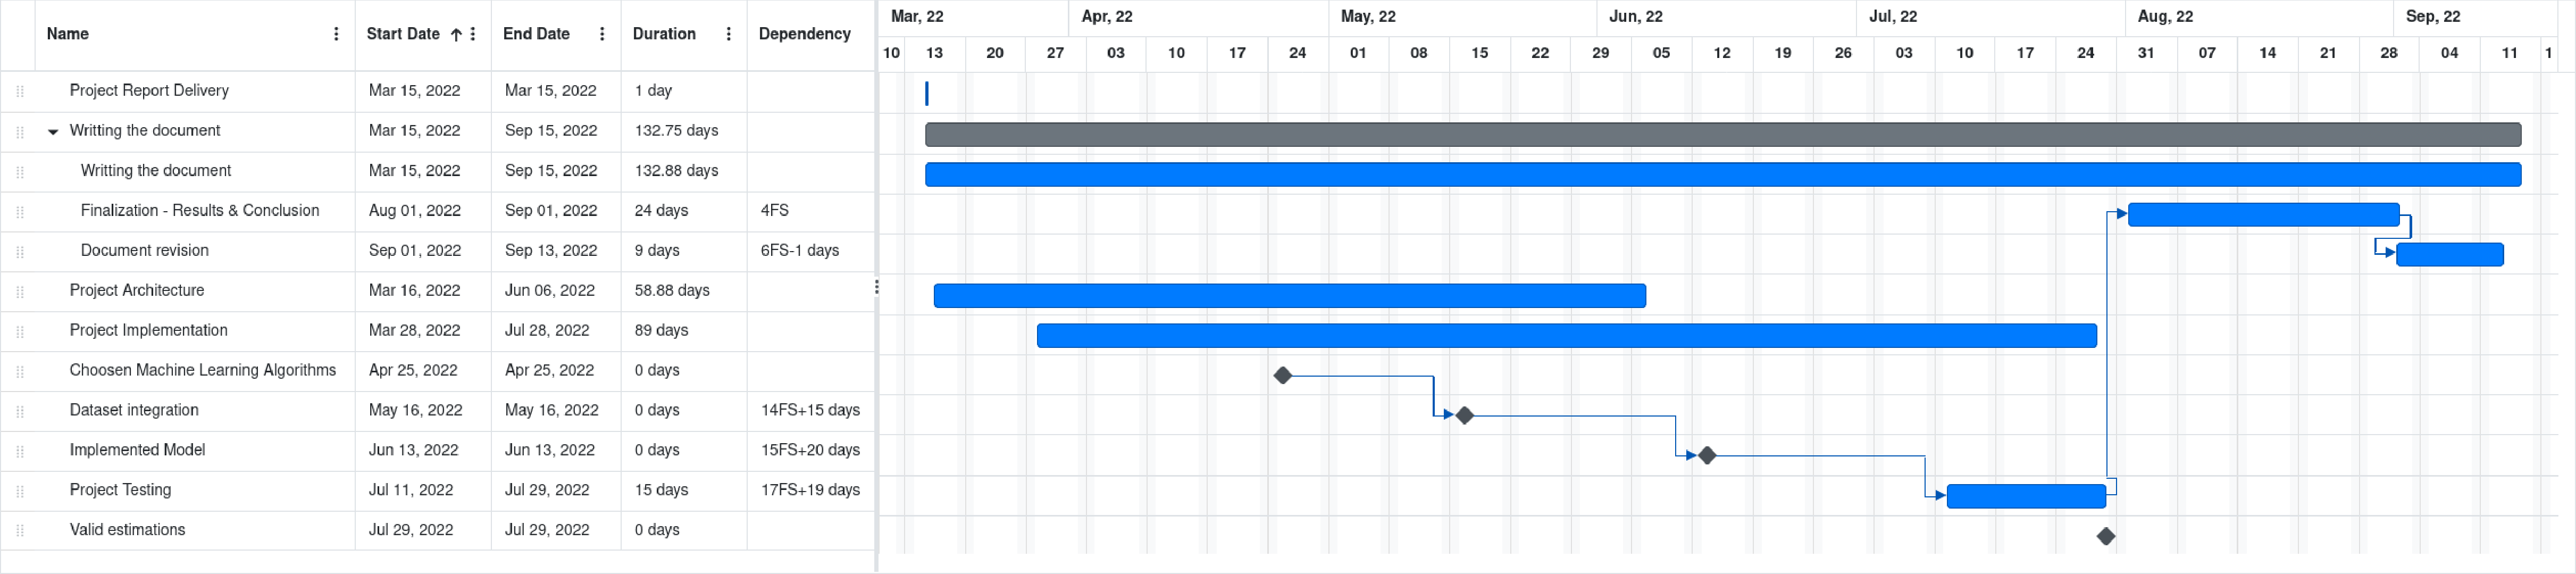
\includegraphics[scale=0.14]{./figures/planning}
        \caption{Project planning.}
    \end{center}
\end{figure}


\end{frame}

\end{document}